\section{Introduction}
\label{sec:introduction}
%
The GIPER instrument consortium answer to the ESA \ac{AO}\cite{JUICE_AO} for the L1 class \ac{JUICE} mission.
%
%
\subsection{JUICE Mission Overview}
ESA L1 mission selected May 2012 in Cosmic Vision programme. Expected launch date 2022. 7.5 year cruise to Jupiter. Orbit insertion 2030 around Jupiter including phase studies of Europa and Callisto. September 2032 orbit insertion around Ganymede. Nominal mission end 2033. Russian Ganymede lander.
%
%
\section{Scientific Objectives}
%scientific investigation. Overall instrument capability, global mission goal, anticipated scientific performance on instrument, compared to similar instruments, discussion of synergies between different observations, list of assuptions for achieving science objectives: SC performance, orbit, other payloads, ground segment.
%
The scientific outcome of this instrument proposal is in accordance with ESA \ac{SciRD}\cite{SciRD} and addresses many of the scientific investigations proposed in the ESA JUICE Assessment Study Report\cite{yellowbook}.
%
%
\subsection{Introduction}
\subsection{Scientific Goals}
\subsection{Scientific Performance Requirements}
% 
%
\section{Instrument Performance}
%sensitivities, assumptions, critical analysis to environement parameters (radiation, degradation etc.), orbit positions.
%

\section{Technical Description and Design}
%
The proposed instrument has been designed in accordance to ESA \ac{EID-A} for the \ac{JUICE} mission\cite{EIDA}.
%
\subsection{Design Overview}
\subsection{Instrument Design Elements}
\subsection{Technical Resources}
\subsection{Instrument Spacecraft Requirements}
%thermal, power, mechanical mounting, EMC, especially radiation sensitive parts, radiation shielding and mitigation strategy, flight heritage of hardware, ressource budgets, 
This mission assumes that an altimeter instrument is included in the JUICE mission scientific instrument package. Altimeter is needed to estimate the surface clutter and surface slope.
%
\section{Summary of Instrument Interfaces}
%data, mechanical, power, EMC, thermal,
%
\section{On-ground and In-flight Test and Calibration}
%test equipment requirements (i.e. thermal vacuum chamber, EMC labs etc.), EGSE, radar signal simulator(test of ground processing chain),
%
Functional, EMC, Thermal-Vacuum, Vibration.
%
%
For \ac{EGSE} a \ac{GIPER} raw signal simulator will be developed by the instrument consortia. The raw signal simulator will be similar to the one developed for the \ac{SHARAD} instrument\cite{Giovanni} and allow testing of the signal processing chain and to develop a Ganymede transfer function considering the orbit altitude and surface clutter and sub-surface dielectric interfaces. 
%
%
\begin{wrapfigure}{r}{0.3\textwidth}
\centering
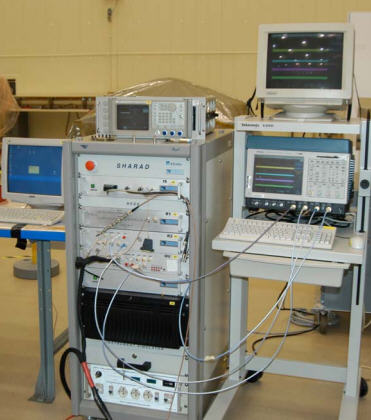
\includegraphics[width=0.27\textwidth]{figures/MEGS}
\caption[caption]{Mars Echo Generation System used on the SHARAD instrument\cite{MEGS}}
\label{fig:MEGS}
\end{wrapfigure}
%
%
In-flight internal calibration (transmitted signal looped to receiver and data sent to ground)
In-flight external calibration (unprocessed data of reflected signals from a flat surface region of Ganymede is sent to ground)
%
%
\section{System Level Assembly, Integration and Verification}
%
%
\subsection{Requirements}
\subsection{Deliverable Models}
%
Two models of the proposed instrument will be developed:
\begin{itemize}
\item Engineering Model - To test and verify the instruments functional and technical requirements as well as the instrument performance.\\
\item Protoflight Model - will be build using full flight standard components and tested at qualification levels.
\end{itemize}
%
\subsection{System Level Testing}
%
\section{Flight Operations Concept}
%operational modes, calibrations, 
%
The instrument modes are inherited from the SHARAD instrument\cite{SHARAD_ppt}.
%
\subsection{Nominal Operations}
%
Operation modes: Low data rate, high data rate, calibration, receive only
%
\subsection{Other Modes}
%
Silent Modes: Off, Heating
Support modes: Check/init, standby, warm-up, idle
%
%
%
\section{Science Ground Segment Concept}
%operations requests, on-board software maintenance (test facilities to generate and test update)
%Further described in the Science Implementation Plan (SIP) - answer to SIRD
\subsection{Implementation concept for the Science Ground Segment}
\subsection{Planning of payload operations}
\subsection{On-Board Software Maintenance}
%
\section{Data Reduction, Scientific Analysis and Archival Plans}
%
\section{Organization}
%\subsection{Schedule}
\subsection{Management Structure}
(Please note, some of the contents in this section are fictive and should not be taken literally.)\\\\
%
\noindent
Dr. Jan Sommer is the instrument \ac{PI}. He has an extensive background studying planet geology, especially on Mars. This study will enhance our knowledge of planet inner structures, geology and provide better understanding of planet formations and evolution.\\\\
%
\noindent
Morten Olsen is the project manager. With experience as project manager for previous successful space instruments, he will manage the project schedules and budgets.\\\\
%
\noindent
Omair Sarwar is the technical manager. With extended engineering experience in radar systems, he will ensure that the instrument meets the performance requirements, proper instrument verification and qualification in accordance with ESA space standards.\\\\
%
\subsection{Budget}
ACME Space Agency is the \ac{LFA} for this instrument proposal. A \ac{LEO} has been issued ensuring funding for the project during the instrument development phase, in-flight operations and post operations activities.